%%% LaTeX Template: Article/Thesis/etc. with colored headings and special fonts
%%%
%%% Source: http://www.howtotex.com/
%%% Feel free to distribute this template, but please keep to referal to http://www.howtotex.com/ here.
%%% February 2011
%%%
%%% Modified May 2018 by CDM

%%%  Preamble
\documentclass[11pt,letterpaper]{article}
\usepackage[margin=1.0in]{geometry}
\usepackage[T1]{fontenc}
\usepackage[bitstream-charter]{mathdesign}
\usepackage[latin1]{inputenc}					
\usepackage{amsmath}						
\usepackage{xcolor}
\usepackage{cite}
\usepackage{hyphenat}
\usepackage{graphicx}
\usepackage{float}
\usepackage{subfigure}
\usepackage{sectsty}
\usepackage[compact]{titlesec} 
\usepackage[tablegrid]{vhistory}
\allsectionsfont{\color{accentcolor}\scshape\selectfont}

%%% Definitions
\definecolor{accentcolor}{rgb}{0.0,0.0,0.5} 
\newcommand{\teamname}{No SHUT Eye}
\newcommand{\productname}{Smart Shutters}
\newcommand{\coursename}{CSE 4316: Senior Design I}
\newcommand{\semester}{Fall 2019}
\newcommand{\docname}{Project Charter}
\newcommand{\department}{Department of Computer Science \& Engineering}
\newcommand{\university}{The University of Texas at Arlington}
\newcommand{\authors}{Atafo Abure \\ David Nquyen \\ Deion Nwaefulu \\ Aditya Rajguru \\ Haris Qureshi}

%%% Headers and footers
\usepackage{fancyhdr}
	\pagestyle{fancy}						% Enabling the custom headers/footers
\usepackage{lastpage}	
	% Header (empty)
	\lhead{}
	\chead{}
	\rhead{}
	% Footer
	\lfoot{\footnotesize \teamname \ - \semester}
	\cfoot{}
	\rfoot{\footnotesize page \thepage\ of \pageref{LastPage}}	% "Page 1 of 2"
	\renewcommand{\headrulewidth}{0.0pt}
	\renewcommand{\footrulewidth}{0.4pt}

%%% Change the abstract environment
\usepackage[runin]{abstract}			% runin option for a run-in title
%\setlength\absleftindent{30pt}			% left margin
%\setlength\absrightindent{30pt}		% right margin
\abslabeldelim{\quad}	
\setlength{\abstitleskip}{-10pt}
\renewcommand{\abstractname}{}
\renewcommand{\abstracttextfont}{\color{accentcolor} \small \slshape}	% slanted text

%%% Start of the document
\begin{document}

%%% Cover sheet
{\centering \huge \color{accentcolor} \sc \textbf{\department \\ \university} \par}
\vspace{1 in}
{\centering \huge \color{accentcolor} \sc \textbf{\docname \\ \coursename \\ \semester} \par}
\vspace{0.5 in}
\vspace{0.5 in}
{\centering \huge \color{accentcolor} \sc \textbf{\teamname \\ \productname} \par}
\vspace{0.5 in}
{\centering \large \sc \textbf{\authors} \par}
\newpage


%\vspace{1 in}
%\centerline{January 13th, 2012}
%\newpage

%%% Revision History
\begin{versionhistory}
  	\vhEntry{0.1}{09.26.2019}{HQ|AA|DN|DN|AR}{document creation}
  	\vhEntry{0.2}{09.30.2019}{AA|HQ|DN|DN|AR}{complete draft}
  	\vhEntry{1.0}{10.01.2018}{AA|HQ|DN|DN|AR}{official release}
\end{versionhistory}
\newpage

%%% Table of contents
\setcounter{tocdepth}{3}
\tableofcontents
\newpage

%%% List of figures and tables (optional)
\listoffigures
%\listoftables
\newpage

\section{Product Concept}
The Smart Shutter is a system that performs the single task of opening and closing shutters either from user input or from a schedule. The intended user audience is eventually everyone but for now it is nursing homes or assisted living. They will be able to interact with the shutters through an app available on either ios or android. On the app users can set a schedule for when the shutters can open or close, and users can open or close the shutters.  

\subsection{Purpose and Use}
We expect our product to be used everyday either following an adjustable schedule or from user input. The shutter should 100\% adjustable meaning if the user only wants the shutters open 10\% or 17\% they can do that. Also if the user decides to adjust the position the app will update and show that new position.

\subsection{Intended Audience}
Currently our intended users are people who live in assisted care, we do plan on going public with the product and it being available in retail stores. This product is designed for all customers not limited to assisted care.


\newpage
\section{Product Description}
This section provides an overview of The Smart Shutter. The primary operational aspects of our product, from the perspective of end users, maintainers and administrators, are defined here. The key features and functions found in the product, as well as critical user interactions and user interfaces are described in detail

\subsection{Features \& Functions}
The Smart Shutters main functionality is to change position remotely according to the users, who will either set a schedule for the shutters to follow or real time user input. The users will interact with the shutters through an app that is available on either android or ios. The app will then communicate to a hub that will then relay the request to each shutter. 


\subsection{External Inputs \& Outputs}
From the users we expect positions, meaning either preset positions or a specific number for how much light the shutter should let in. From the system we expect a few outputs such as an acknowledgement for receiving the request and completed the request, then it will state the new position of the shutters and the battery level. 

\subsection{Product Interfaces}
\begin{figure}[H]
    \centering
    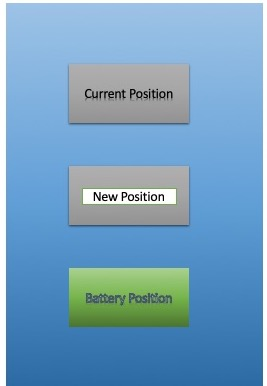
\includegraphics[width=0.5\textwidth]{images/ChangePosition}
    \caption{Change Position Interface}
\end{figure}
\begin{figure}[H]
    \centering
    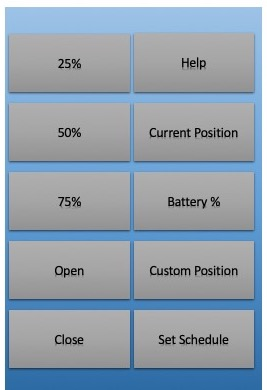
\includegraphics[width=0.5\textwidth]{images/HomeScreen}
    \caption{Home Screen Interface}
\end{figure}
\newpage
\section{Customer Requirements}
Some of our customer requirements are the product has to open and close, to be easy to set up, battery powered, ready for large scale production, Bluetooth/WiFi controlled, and be \$20 or less. Other products that are available on the market do meet some of these requirements but all those products are not around \$20. Our focus is being around \$20 while in low level production, this way when we scale up it will lower cost due to buying parts in bulk. Another one of the requirements is the product being easy to set up. This means the customer set up experience should last around 5 to 10 minutes. The customer should be able to remotely control the shutters from almost anywhere in the building, basements may not work.

\subsection{Cost \$20 Shipped}
\subsubsection{Description}
The device has to cost the customer \$20 to buy. This is a critical requirement for our product, if we do not meet this we will start over.

\subsubsection{Source}
Sponsor
\subsubsection{Constraints}
It all depends on our microcontroller, motor, motor controller, wifi or bluetooth adapter, it depends on the price of each of those components.

\subsubsection{Standards}
No standards for pricing
\subsubsection{Priority}
Critical

\subsection{Bluetooth and Wi-Fi Connectivity}
\subsubsection{Description}
The Hub should be able to communicate with a remote over Wi-Fi and connect to the shutters over Bluetooth.

\subsubsection{Source}
Sponsor
\subsubsection{Constraints}
Bluetooth normally has a one to one relationship with slave and master and can not be controlled from anywhere, while WiFi can have multiple devices on one network and can be controlled from anywhere in the world.


\subsubsection{Standards}
IEEE 802.11
IEEE 802.15.2

\subsubsection{Priority}
Critical

\subsection{Easy Set Up}
\subsubsection{Description}
The setup process should take only 5 minutes and be easy low number of steps 


\subsubsection{Source}
Sponsor
\subsubsection{Constraints}
All depends on our ability for setting up communication


\subsubsection{Standards}
IEEE 1233
\subsubsection{Priority}
High

\subsection{Opening and Closing}
\subsubsection{Description}
This is a critical requirement for our product, if the product can not open and close or open a certain percentage we will have to start over.

\subsubsection{Source}
Sponsor
\subsubsection{Constraints}
Has to open and close automatically, following a schedule, or from remote input 

\subsubsection{Standards}
No standards for this requirement
\subsubsection{Priority}
Critical



\newpage
\section{Packaging Requirements}
The package that will be delivered to the customer will contain the following the smart shutter including the motor, a set of batteries, and  a QR code which will redirect users to the website where they can download the app on their mobile device.

\subsection{Smart Shutter}
\subsubsection{Description}
Shutters that able to be remotely adjusted from anywhere in the building and is battery powered.
\subsubsection{Source}
Sponsor
\subsubsection{Constraints}
Physical size of the shutters
\subsubsection{Standards}
Federal Trade Commission Packaging requirements 
\subsubsection{Priority}
Critical

\subsection{Battery}
\subsubsection{Description}
The smart shutters will run on battery power, this a very important piece in our product.

\subsubsection{Source}
Sponsor
\subsubsection{Constraints}
Handling of the package, temperature and physical size
\subsubsection{Standards}
Federal Trade Commission Packaging requirements, environmental protection agency requirements
\subsubsection{Priority}
Critical

Federal Trade Commission Packaging requirements, environmental protection agency requirements

\newpage
\section{Performance Requirements}
Performance requirements for our product include remote control, set up time should take within 5 minutes, and inputs should be handled and successfully completed within 30 seconds


\subsection{Remote Control}
\subsubsection{Description}
Smart shutters must take input remotely 
\subsubsection{Source}
Sponsor
\subsubsection{Constraints}
Programmers knowledge and skills.
\subsubsection{Standards}
IEEE 802.11 and IEEE 802.15.4
\subsubsection{Priority}
Critical

\subsection{Quick Installation}
\subsubsection{Description}
Smart shutters must take input remotely 
\subsubsection{Source}
Sponsor
\subsubsection{Constraints}
Programmers knowledge and skills.
\subsubsection{Standards}
IEEE 802.11 and IEEE 802.15.4
\subsubsection{Priority}
Critical

\subsection{Input Handling}
\subsubsection{Description}
Input should be correctly handled with in 30 seconds 
\subsubsection{Source}
Sponsor
\subsubsection{Constraints}
Programmers knowledge and skills.
\subsubsection{Standards}
IEEE 802.11 and IEEE 802.15.4
\subsubsection{Priority}
Critical
\newpage
\section{Safety Requirements}
The product shall have very little to no sharp edges that shall harm a user, The product shall also have all electrical connections grounded to avoid shock

\subsection{Laboratory equipment lockout/tagout (LOTO) procedures}
\subsubsection{Description}
Any fabrication equipment provided used in the development of the project shall be used in accordance with OSHA standard LOTO procedures. Locks and tags are installed on all equipment items that present use hazards, and ONLY the course instructor or designated teaching assistants may remove a lock. All locks will be immediately replaced once the equipment is no longer in use.
\subsubsection{Source}
CSE Senior Design laboratory policy
\subsubsection{Constraints}
Equipment usage, due to lock removal policies, will be limited to availability of the course instructor and designed teaching assistants.
\subsubsection{Standards}
Occupational Safety and Health Standards 1910.147 - The control of hazardous energy (lockout/tagout).
\subsubsection{Priority}
Critical

\subsection{National Electric Code (NEC) wiring compliance}
\subsubsection{Description}
Any electrical wiring must be completed in compliance with all requirements specified in the National Electric Code. This includes wire runs, insulation, grounding, enclosures, over-current protection, and all other specifications.
\subsubsection{Source}
CSE Senior Design laboratory policy
\subsubsection{Constraints}
High voltage power sources, as defined in NFPA 70, will be avoided as much as possible in order to minimize potential hazards.
\subsubsection{Standards}
NFPA 70
\subsubsection{Priority}
Critical

\subsection{RIA robotic manipulator safety standards}
\subsubsection{Description}
Robotic manipulators, if used, will either housed in a compliant lockout cell with all required safety interlocks, or certified as a "collaborative" unit from the manufacturer.
\subsubsection{Source}
CSE Senior Design laboratory policy
\subsubsection{Constraints}
Collaborative robotic manipulators will be preferred over non-collaborative units in order to minimize potential hazards. Sourcing and use of any required safety interlock mechanisms will be the responsibility of the engineering team.
\subsubsection{Standards}
ANSI/RIA R15.06-2012 American National Standard for Industrial Robots and Robot Systems, RIA TR15.606-2016 Collaborative Robots
\subsubsection{Priority}
Critical

\newpage
\section{Maintenance \& Support Requirements}
For the support we will be providing a frequently asked questions section on the website for users, all documentation for the code will be available on the website, the code will be handed over to the sponsor after product delivery and the group in charge of production will handle the maintenance after the delivery of the product.

\subsection{FAQ}
\subsubsection{Description}
Frequently asked questions are posted on company website intended to help other customers with similar issues or questions.
\subsubsection{Source}
Sponsor
\subsubsection{Constraints}
Providing effective feedback and quickly
\subsubsection{Standards}
Business Communication standards 
\subsubsection{Priority}
 Critical
 
 \subsection{iOS and Android App Support}
\subsubsection{Description}
If there are any bugs with the app users will submit a request on either the app or FAQ and our technical support team will contact them or they can contact technical support
 similar issues or questions.
\subsubsection{Source}
Sponsor
\subsubsection{Constraints}
Providing effective support and quickly
\subsubsection{Standards}
Business Communication standards 
\subsubsection{Priority}
 Critical
\newpage
\section{Other Requirements}
Other requirements include there being apps for both android and ios and the code being modular so each section can act independently and be changed without having to change the entirety of the code base.

\subsection{Android App}
\subsubsection{Description}
Blink shutters mobile application that lets users interact with their smart shutter appliance. Includes setting a schedule for when the shutters will open and how much light will they let in, it will also display the each shutters battery percentage and the current position the shutters are in.
\subsubsection{Source}
Sponsor
\subsubsection{Constraints}
Programmers skills and time
\subsubsection{Standards}
IEEE 802.11 and IEEE 802.15
\subsubsection{Priority}
Critical

\subsection{iOS App}
\subsubsection{Description}
Blink shutters mobile application that lets users interact with their smart shutter appliance. Includes setting a schedule for when the shutters will open and how much light will they let in, it will also display the each shutters battery percentage and the current position the shutters are in.

\subsubsection{Source}
Sponsor
\subsubsection{Constraints}
Programmers skills and time
\subsubsection{Standards}
IEEE 802.11 and IEEE 802.15
\subsubsection{Priority}
Critical

\subsection{Modular Code }
\subsubsection{Description}
Each section of the program must be completely independent of each other. Meaning if we change the embedded code for the shutters this should not affect how we send information to the app through the middle where. This will also help in locating bugs and should lead to them being fixed quicker.

\subsubsection{Source}
Sponsor
\subsubsection{Constraints}
Programmers skills and time
\subsubsection{Standards}
IEEE 802.11 and IEEE 802.15
\subsubsection{Priority}
Critical
\newpage
\section{Future Items}

\subsection{Apple Homekit and smart assistant integration}
\subsubsection{Description}
In the future all shutters should be able to be controlled from a device with the help of a smart assistant command
\subsubsection{Source}
Sponsor
\subsubsection{Constraints}
Programmers knowledge and skills
\subsubsection{Standards}
IEEE 802.11 and 802.15.4
\subsubsection{Priority}
High
\newpage

%%% References
\bibliographystyle{plain}
\bibliographystyle{reference/IEEEtran_custom}
\bibliography{reference/refs}{}

\end{document}